%%%%%%%%%%%%%%%%%%%%%%%%%%%%%%%%%%%%%%%%%%%%%%%%%%%%%%%%%%%%%%%%%%%%%%%%%%%%%%%%%%
\begin{frame}[fragile]\frametitle{}
\begin{center}
{\Large Implementations}
\end{center}
\end{frame}

%%%%%%%%%%%%%%%%%%%%%%%%%%%%%%%%%%%%%%%%%%%%%%%%%%%%%%%%%%%%%%%%%%%%%%%%%%%%%%%%%%
\begin{frame}[fragile]\frametitle{}
\begin{center}
{\Large Crew AI}
\end{center}
\end{frame}

%%%%%%%%%%%%%%%%%%%%%%%%%%%%%%%%%%%%%%%%%%%%%%%%%%%%%%%%%%%
\begin{frame}[fragile]\frametitle{Introduction to CrewAI}
      \begin{itemize}
        \item Build AI agent teams that work together to tackle complex tasks
        \item Enables collaborative intelligence between specialized AI agents
        \item Designed for autonomous operation with human-like team coordination
        \item Empowers developers to create sophisticated AI automation systems
        \item Over 100,000 developers certified through community courses
        \item Rapidly becoming the standard for enterprise-ready AI automation
      \end{itemize}
\end{frame}

%%%%%%%%%%%%%%%%%%%%%%%%%%%%%%%%%%%%%%%%%%%%%%%%%%%%%%%%%%%
\begin{frame}[fragile]\frametitle{What is CrewAI?}
      \begin{itemize}
        \item Open-source framework to manage AI agents
		\item Orchestration like real world teams
		\item Each agent has role, responsibilities and is expected to get things done.
        \item Lean, lightning-fast Python framework built entirely from scratch
        \item Completely independent of LangChain or other agent frameworks
        \item Provides both high-level simplicity and precise low-level control
        \item Ideal for creating autonomous AI agents tailored to any scenario
        \item Two main components: CrewAI Crews and CrewAI Flows
        \item Crews optimize for autonomy and collaborative intelligence
        \item Flows enable granular, event-driven control for precise orchestration
        \item Supports single LLM calls and native Crews integration
      \end{itemize}
\end{frame}



%%%%%%%%%%%%%%%%%%%%%%%%%%%%%%%%%%%%%%%%%%%%%%%%%%%%%%%%%%%%%%%%%%%%%%%%%%%%%%%%%%
\begin{frame}[fragile]\frametitle{What So Special?}
    \begin{itemize}
        \item Role-based architecture
		\item Collaborative tasks handling
		\item Goal-driven execution
		\item Iterative thinking and feedback loops
		\item Communication between agents
    \end{itemize}
	
	
\end{frame}

%%%%%%%%%%%%%%%%%%%%%%%%%%%%%%%%%%%%%%%%%%%%%%%%%%%%%%%%%%%%%%%%%%%%%%%%%%%%%%%%%%
\begin{frame}[fragile]\frametitle{Building blocks}

Define:
    \begin{itemize}
        \item Role: like Researcher, Writer, etc using system prompt
		\item Tasks: What each agent needs to accomplish
		\item Agents: equipped with LLMs, Memory, role and tools
		\item Crew: team of agents working together
    \end{itemize}
	
		\begin{center}
		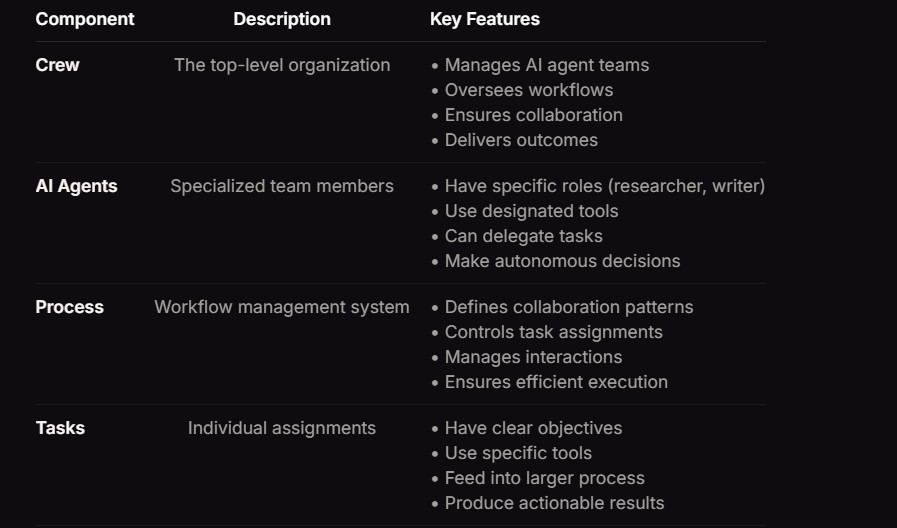
\includegraphics[width=0.7\linewidth,keepaspectratio]{crewai2}
		
		{\tiny (Ref: Crew AI documentation)}	
		\end{center}		
		
\end{frame}

%%%%%%%%%%%%%%%%%%%%%%%%%%%%%%%%%%%%%%%%%%%%%%%%%%%%%%%%%%%
\begin{frame}[fragile]\frametitle{How Crews Work?}
      \begin{itemize}
        \item The Crew organizes the overall operation
        \item AI Agents work on their specialized tasks
        \item The Process ensures smooth collaboration
        \item Tasks get completed to achieve the goal
      \end{itemize}
	  
		\begin{center}
		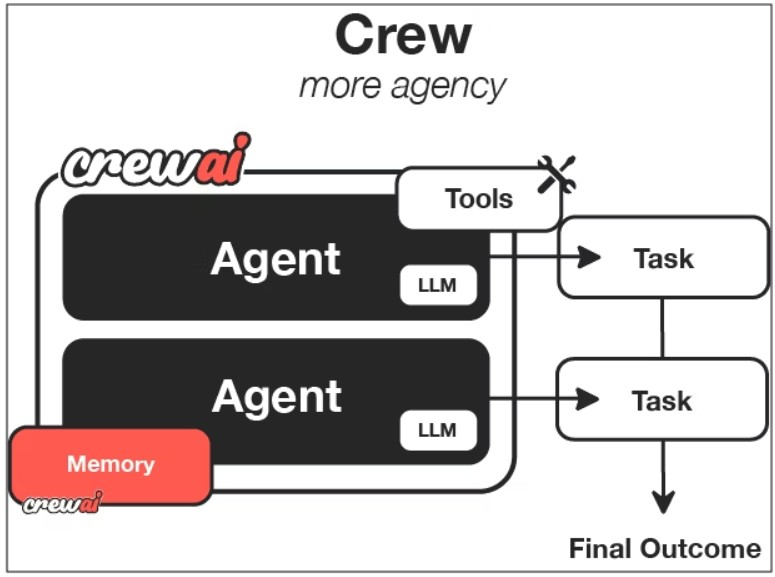
\includegraphics[width=0.55\linewidth,keepaspectratio]{crewai1}
		
		{\tiny (Ref: Crew AI documentation)}
		\end{center}		  
\end{frame}
		
%%%%%%%%%%%%%%%%%%%%%%%%%%%%%%%%%%%%%%%%%%%%%%%%%%%%%%%%%%%
\begin{frame}[fragile]\frametitle{How Crews Work - Company Analogy}
      \begin{itemize}
        \item Similar to company departments (Sales, Engineering, Marketing)
        \item Departments work together under leadership to achieve business goals
        \item CrewAI creates an organization of AI agents with specialized roles
        \item Agents collaborate to accomplish complex tasks autonomously
        \item Each agent has specific responsibilities and expertise areas
        \item Leadership structure ensures coordination and goal alignment
        \item Enables division of labor for efficient task completion
      \end{itemize}
\end{frame}

% %%%%%%%%%%%%%%%%%%%%%%%%%%%%%%%%%%%%%%%%%%%%%%%%%%%%%%%%%%%
% \begin{frame}[fragile]\frametitle{CrewAI Core Components}
      % \begin{itemize}
        % \item \textbf{Crew}: Top-level organization managing AI agent teams
        % \item \textbf{AI Agents}: Specialized team members with specific roles
        % \item \textbf{Process}: Workflow management system defining collaboration patterns
        % \item \textbf{Tasks}: Individual assignments with clear objectives
        % \item Crew oversees workflows and ensures collaboration
        % \item Agents use designated tools and make autonomous decisions
        % \item Process controls task assignments and manages interactions
        % \item Tasks feed into larger processes to produce actionable results
      % \end{itemize}
% \end{frame}

% %%%%%%%%%%%%%%%%%%%%%%%%%%%%%%%%%%%%%%%%%%%%%%%%%%%%%%%%%%%
% \begin{frame}[fragile]\frametitle{Crew Workflow Integration}
      % \begin{itemize}
        % \item The Crew organizes the overall operation and strategy
        % \item AI Agents work on their specialized tasks independently
        % \item The Process ensures smooth collaboration between agents
        % \item Tasks get completed systematically to achieve the goal
        % \item Agents can delegate tasks and communicate with each other
        % \item Workflow ensures efficient execution and resource utilization
        % \item Results are aggregated to deliver comprehensive outcomes
      % \end{itemize}
% \end{frame}

% %%%%%%%%%%%%%%%%%%%%%%%%%%%%%%%%%%%%%%%%%%%%%%%%%%%%%%%%%%%
% \begin{frame}[fragile]\frametitle{How Flows Work}
      % \begin{itemize}
        % \item Crews excel at autonomous collaboration
        % \item Flows provide structured automations with granular control
        % \item Ensure tasks are executed reliably, securely, and efficiently
        % \item Handle conditional logic, loops, and dynamic state management
        % \item Provide precision control over workflow execution paths
        % \item Integrate seamlessly with Crews for balanced automation
        % \item Balance high autonomy with exacting control requirements
        % \item Enable structured workflows with intelligent decision points
      % \end{itemize}
	  
		% \begin{center}
		% 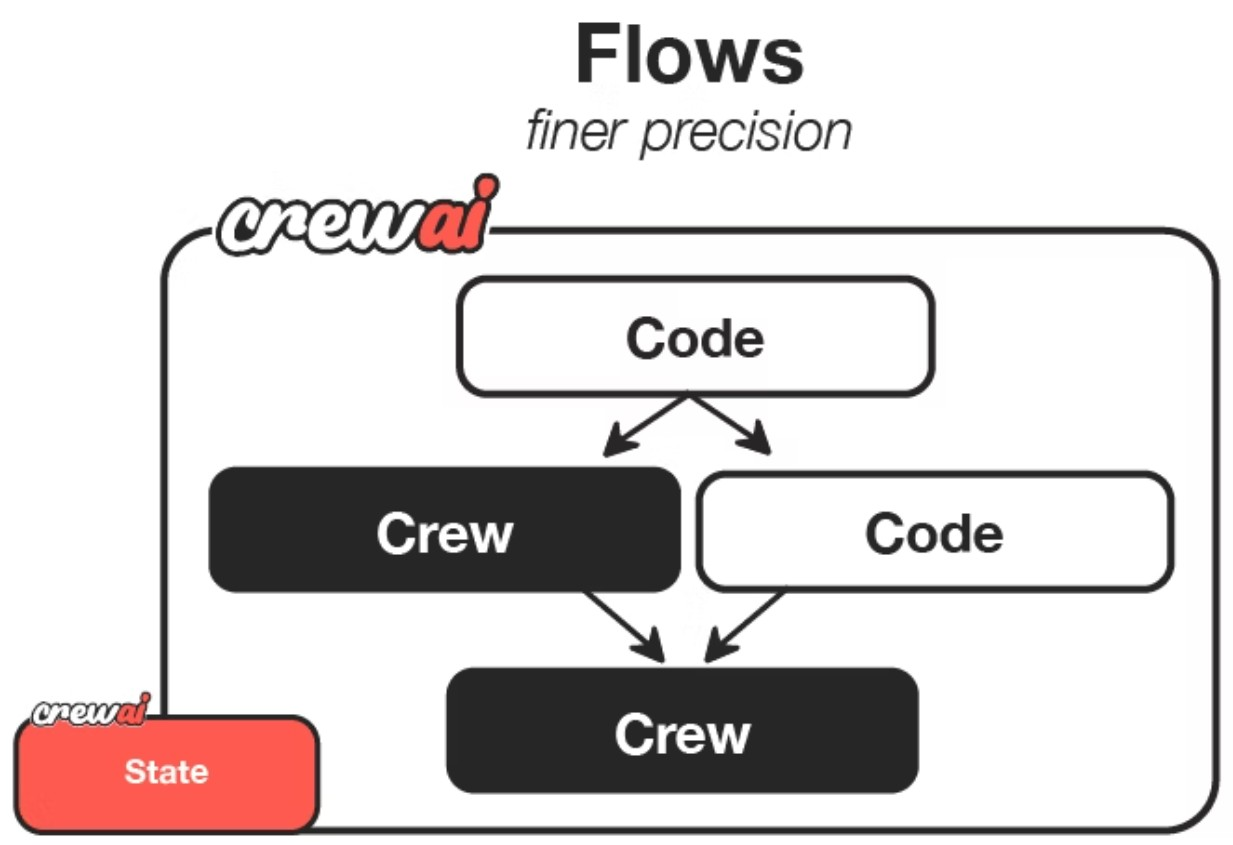
\includegraphics[width=0.6\linewidth,keepaspectratio]{crewai3}
		
		% {\tiny (Ref: Crew AI documentation)}
		% \end{center}		

% \end{frame}

% %%%%%%%%%%%%%%%%%%%%%%%%%%%%%%%%%%%%%%%%%%%%%%%%%%%%%%%%%%%
% \begin{frame}[fragile]\frametitle{Flow Components Breakdown}
      % \begin{itemize}
        % \item \textbf{Flow}: Structured workflow orchestration managing execution paths
        % \item \textbf{Events}: Triggers for workflow actions enabling dynamic responses
        % \item \textbf{States}: Workflow execution contexts maintaining execution data
        % \item \textbf{Crew Support}: Enhances workflow automation with pockets of agency
        % \item Flows handle state transitions and control task sequencing
        % \item Events support conditional branching and real-time adaptation
        % \item States enable persistence, resumability, and execution integrity
        % \item Crew Support balances automation with intelligent decision-making
      % \end{itemize}
	  
		% \begin{center}
		% 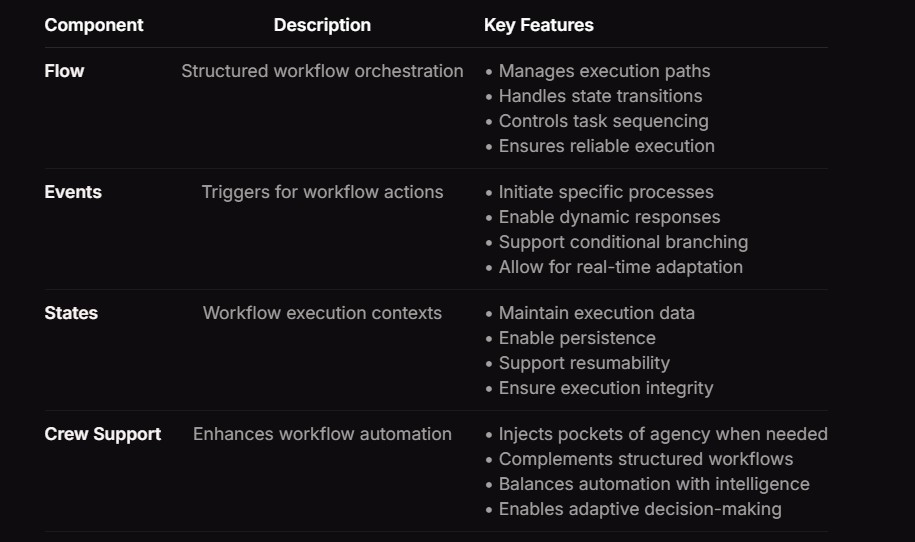
\includegraphics[width=0.6\linewidth,keepaspectratio]{crewai4}
		
		% {\tiny (Ref: Crew AI documentation)}
		% \end{center}		
		
% \end{frame}

% %%%%%%%%%%%%%%%%%%%%%%%%%%%%%%%%%%%%%%%%%%%%%%%%%%%%%%%%%%%
% \begin{frame}[fragile]\frametitle{Crews vs Flows - Use Cases}
      % \begin{itemize}
        % \item \textbf{Open-ended research}: Use Crews for creative thinking and exploration
        % \item \textbf{Content generation}: Use Crews for collaborative article creation
        % \item \textbf{Decision workflows}: Use Flows for predictable, auditable paths
        % \item \textbf{API orchestration}: Use Flows for reliable external service integration
        % \item \textbf{Hybrid applications}: Combine both approaches strategically
        % \item Flows orchestrate overall process while Crews handle complex subtasks
        % \item Choose based on autonomy needs vs. control requirements
      % \end{itemize}
	  
		% \begin{center}
		% 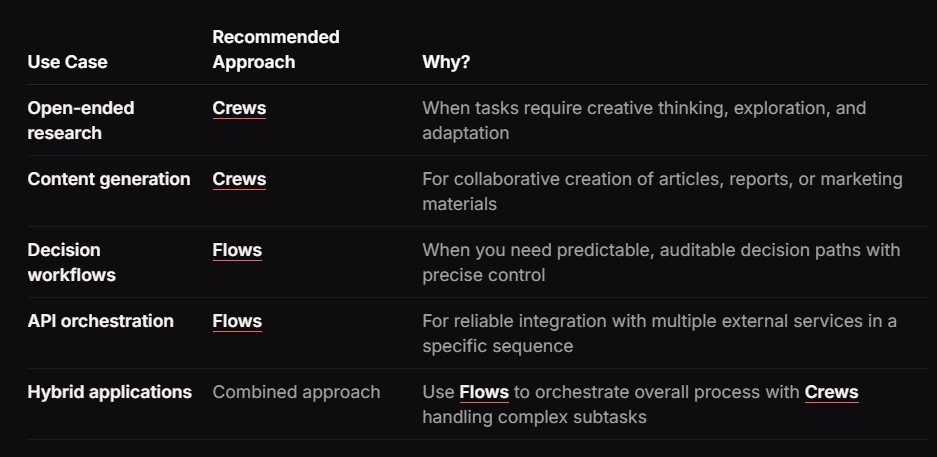
\includegraphics[width=0.6\linewidth,keepaspectratio]{crewai5}
		
		% {\tiny (Ref: Crew AI documentation)}
		% \end{center}			  
% \end{frame}

% %%%%%%%%%%%%%%%%%%%%%%%%%%%%%%%%%%%%%%%%%%%%%%%%%%%%%%%%%%%
% \begin{frame}[fragile]\frametitle{Decision Framework}
      % \begin{itemize}
        % \item \textbf{Choose Crews when}: Autonomous problem-solving is required
        % \item Need creative collaboration or exploratory tasks
        % \item Tasks require adaptation and flexible thinking approaches
        % \item \textbf{Choose Flows when}: Deterministic outcomes are essential
        % \item Require auditability and precise control over execution
        % \item Need reliable, repeatable processes with minimal variation
        % \item \textbf{Combine both when}: Application needs structured processes
        % \item Require pockets of autonomous intelligence within controlled workflows
      % \end{itemize}
% \end{frame}


%%%%%%%%%%%%%%%%%%%%%%%%%%%%%%%%%%%%%%%%%%%%%%%%%%%%%%%%%%%%%%%%%%%%%%%%%%%%%%%%%%
\begin{frame}[fragile]\frametitle{Applications}

Examples:
    \begin{itemize}
        \item AI Agents for Equity Research using tools to call APIs, MCP servers
		\item Multi-Agent support bots: Classifier $\rightarrow$ Specialized Agents $\rightarrow$ Compose response.
		\item Agentic Workflows
		\item Etc.
    \end{itemize}
\end{frame}


%%%%%%%%%%%%%%%%%%%%%%%%%%%%%%%%%%%%%%%%%%%%%%%%%%%%%%%%%%%%%%%%%%%%%%%%%%%%%%%%%%
\begin{frame}[fragile]\frametitle{}
\begin{center}
{\Large Demo of Crew AI}
\end{center}
\end{frame}

%%%%%%%%%%%%%%%%%%%%%%%%%%%%%%%%%%%%%%%%%%%%%%%%%%%%%%%%%%%%%%%%%%%%%%%%%%%%%%%%%%
\begin{frame}[fragile]\frametitle{Install CrewAI }

Ensure you have Python $>=3.10 <3.14$

Install uv

Install CrewAI 

    \begin{lstlisting}
powershell -ExecutionPolicy ByPass -c "irm https://astral.sh/uv/install.ps1 | iex"	
# pip install crewai

uv tool install crewai

uv tool list

    \end{lstlisting}			
\end{frame}


%%%%%%%%%%%%%%%%%%%%%%%%%%%%%%%%%%%%%%%%%%%%%%%%%%%%%%%%%%%%%%%%%%%%%%%%%%%%%%%%%%
\begin{frame}[fragile]\frametitle{Creating a CrewAI Project}

Use the YAML template scaffolding for a structured approach to defining agents and tasks. Here’s how to get started \lstinline|crewai create crew <your_project_name>|


		\begin{center}
		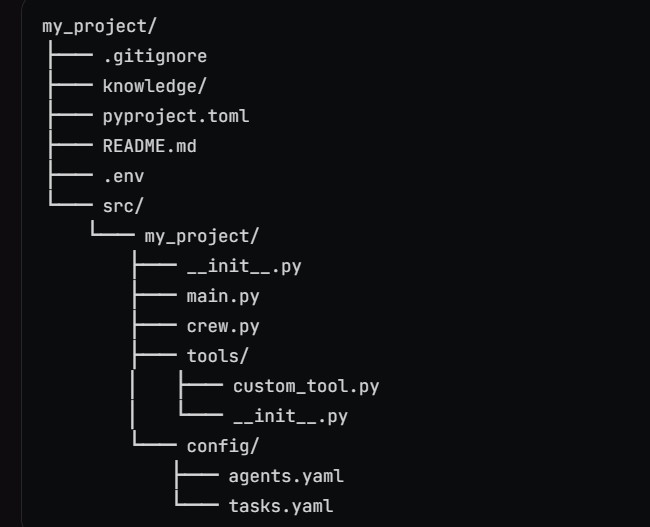
\includegraphics[width=0.45\linewidth,keepaspectratio]{crewai7}
		\end{center}
		
Run your Crew		
    \begin{lstlisting}
crewai install
crewai run
    \end{lstlisting}			
\end{frame}


%%%%%%%%%%%%%%%%%%%%%%%%%%%%%%%%%%%%%%%%%%%%%%%%%%%%%%%%%%%%%%%%%%%%%%%%%%%%%%%%%%
\begin{frame}[fragile]\frametitle{To customize your project, you can:}

    \begin{itemize}
        \item Modify \lstinline|src/my_project/config/agents.yaml| to define your agents.
        \item Modify \lstinline|src/my_project/config/tasks.yaml| to define your tasks.
        \item Modify \lstinline|src/my_project/crew.py| to add your own logic, tools, and specific arguments.
        \item Modify \lstinline|src/my_project/main.py| to add custom inputs for your agents and tasks.
        \item Add your environment variables into the .env file.
    \end{itemize}
\end{frame}


%%%%%%%%%%%%%%%%%%%%%%%%%%%%%%%%%%%%%%%%%%%%%%%%%%%%%%%%%%%%%%%%%%%%%%%%%%%%%%%%%%
\begin{frame}[fragile]\frametitle{Build your first CrewAI Research Agent}

    \begin{lstlisting}
crewai create crew latest-ai-development
cd latest-ai-development

## Modify your `agents.yaml` file
# src/latest_ai_development/config/agents.yaml
researcher:
  role: >
    {topic} Senior Data Researcher
  goal: >
    Uncover cutting-edge developments in {topic}
  backstory: >
    You're a seasoned researcher with a knack for uncovering the latest
    developments in {topic}. Known for your ability to find the most relevant
    information and present it in a clear and concise manner.
    \end{lstlisting}	
\end{frame}


%%%%%%%%%%%%%%%%%%%%%%%%%%%%%%%%%%%%%%%%%%%%%%%%%%%%%%%%%%%%%%%%%%%%%%%%%%%%%%%%%%
\begin{frame}[fragile]\frametitle{Define Reporting CrewAI Agent}


    \begin{lstlisting}
reporting_analyst:
  role: >
    {topic} Reporting Analyst
  goal: >
    Create detailed reports based on {topic} data analysis and research findings
  backstory: >
    You're a meticulous analyst with a keen eye for detail. You're known for
    your ability to turn complex data into clear and concise reports, making
    it easy for others to understand and act on the information you provide.
    \end{lstlisting}	
\end{frame}

%%%%%%%%%%%%%%%%%%%%%%%%%%%%%%%%%%%%%%%%%%%%%%%%%%%%%%%%%%%%%%%%%%%%%%%%%%%%%%%%%%
\begin{frame}[fragile]\frametitle{Modify your `tasks.yaml` file}


    \begin{lstlisting}
# src/latest_ai_development/config/tasks.yaml
research_task:
  description: >
    Conduct a thorough research about {topic}
    Make sure you find any interesting and relevant information given
    the current year is 2025.
  expected_output: >
    A list with 10 bullet points of the most relevant information about {topic}
  agent: researcher

reporting_task:
  description: >
    Review the context you got and expand each topic into a full section for a report.
    Make sure the report is detailed and contains any and all relevant information.
  expected_output: >
    A fully fledge reports with the mains topics, each with a full section of information.
    Formatted as markdown without '```'
  agent: reporting_analyst
  output_file: report.md
    \end{lstlisting}	
\end{frame}

%%%%%%%%%%%%%%%%%%%%%%%%%%%%%%%%%%%%%%%%%%%%%%%%%%%%%%%%%%%%%%%%%%%%%%%%%%%%%%%%%%
\begin{frame}[fragile]\frametitle{Modify your `crew.py` file}


    \begin{lstlisting}
from crewai import Agent, Crew, Process, Task
from crewai.project import CrewBase, agent, crew, task
from crewai_tools import SerperDevTool
from crewai.agents.agent_builder.base_agent import BaseAgent
from typing import List

@CrewBase
class LatestAiDevelopmentCrew():
  agents: List[BaseAgent]
  tasks: List[Task]

  @agent
  def researcher(self) -> Agent:
    return Agent(
      config=self.agents_config['researcher'], # type: ignore[index]
      verbose=True,
      tools=[SerperDevTool()])

  @agent
  def reporting_analyst(self) -> Agent:
    return Agent(
      config=self.agents_config['reporting_analyst'], # type: ignore[index]
      verbose=True)
    \end{lstlisting}	
\end{frame}

%%%%%%%%%%%%%%%%%%%%%%%%%%%%%%%%%%%%%%%%%%%%%%%%%%%%%%%%%%%%%%%%%%%%%%%%%%%%%%%%%%
\begin{frame}[fragile]\frametitle{Modify your `crew.py` file}


    \begin{lstlisting}
# src/latest_ai_development/crew.py

  @task
  def research_task(self) -> Task:
    return Task(
      config=self.tasks_config['research_task'], # type: ignore[index])

  @task
  def reporting_task(self) -> Task:
    return Task(
      config=self.tasks_config['reporting_task'], # type: ignore[index]
      output_file='output/report.md' # This is the file that will be contain the final report.)

  @crew
  def crew(self) -> Crew:
    """Creates the LatestAiDevelopment crew"""
    return Crew(
      agents=self.agents, # Automatically created by the @agent decorator
      tasks=self.tasks, # Automatically created by the @task decorator
      process=Process.sequential,
      verbose=True,)
    \end{lstlisting}	
\end{frame}


%%%%%%%%%%%%%%%%%%%%%%%%%%%%%%%%%%%%%%%%%%%%%%%%%%%%%%%%%%%%%%%%%%%%%%%%%%%%%%%%%%
\begin{frame}[fragile]\frametitle{[Optional] Add before and after crew functions}


    \begin{lstlisting}
# src/latest_ai_development/crew.py
from crewai import Agent, Crew, Process, Task
from crewai.project import CrewBase, agent, crew, task, before_kickoff, after_kickoff
from crewai_tools import SerperDevTool

@CrewBase
class LatestAiDevelopmentCrew():
  """LatestAiDevelopment crew"""

  @before_kickoff
  def before_kickoff_function(self, inputs):
    print(f"Before kickoff function with inputs: {inputs}")
    return inputs # You can return the inputs or modify them as needed

  @after_kickoff
  def after_kickoff_function(self, result):
    print(f"After kickoff function with result: {result}")
    return result # You can return the result or modify it as needed

  # ... remaining code
    \end{lstlisting}	
\end{frame}

%%%%%%%%%%%%%%%%%%%%%%%%%%%%%%%%%%%%%%%%%%%%%%%%%%%%%%%%%%%%%%%%%%%%%%%%%%%%%%%%%%
\begin{frame}[fragile]\frametitle{Pass custom inputs}

Feel free to pass custom inputs to your crew. For example, you can pass the topic input to your crew to customize the research and reporting.
    \begin{lstlisting}
#!/usr/bin/env python
# src/latest_ai_development/main.py
import sys
from latest_ai_development.crew import LatestAiDevelopmentCrew

def run():
  """
  Run the crew.
  """
  inputs = {
    'topic': 'AI Agents'
  }
  LatestAiDevelopmentCrew().crew().kickoff(inputs=inputs)
    \end{lstlisting}	
\end{frame}

%%%%%%%%%%%%%%%%%%%%%%%%%%%%%%%%%%%%%%%%%%%%%%%%%%%%%%%%%%%%%%%%%%%%%%%%%%%%%%%%%%
\begin{frame}[fragile]\frametitle{Set ENV variables and run}

Set your environment variables in your .env file:
    \begin{lstlisting}
SERPER_API_KEY=YOUR_KEY_HERE

:
:

crewai install
crewai run
    \end{lstlisting}	
\end{frame}

%%%%%%%%%%%%%%%%%%%%%%%%%%%%%%%%%%%%%%%%%%%%%%%%%%%%%%%%%%%%%%%%%%%%%%%%%%%%%%%%%%
\begin{frame}[fragile]\frametitle{Build your first CrewAI Agent}

View your final report in report.md
    \begin{lstlisting}
# Comprehensive Report on the Rise and Impact of AI Agents in 2025

## 1. Introduction to AI Agents
In 2025, Artificial Intelligence (AI) agents are at the forefront of innovation across various industries. As intelligent systems that can perform tasks typically requiring human cognition, AI agents are paving the way for significant advancements in operational efficiency, decision-making, and overall productivity within sectors like Human Resources (HR) and Finance. This report aims to detail the rise of AI agents, their frameworks, applications, and potential implications on the workforce.
:
:
## 8. Conclusion
The emergence of AI agents is undeniably reshaping the workplace landscape in 5. With their ability to automate tasks, enhance efficiency, and improve decision-making, AI agents are critical in driving operational success. Organizations must embrace and adapt to AI developments to thrive in an increasingly digital business environment.
    \end{lstlisting}	
\end{frame}


%%%%%%%%%%%%%%%%%%%%%%%%%%%%%%%%%%%%%%%%%%%%%%%%%%%%%%%%%%%
\begin{frame}[fragile]\frametitle{Why Choose CrewAI?}
      \begin{itemize}
        \item \textbf{Autonomous Operation}: Agents make intelligent role-based decisions
        \item \textbf{Natural Interaction}: Agents communicate like human team members
        \item \textbf{Extensible Design}: Easy to add new tools, roles, and capabilities
        \item \textbf{Production Ready}: Built for reliability and real-world scalability
        \item \textbf{Security-Focused}: Designed with enterprise security requirements
        \item \textbf{Cost-Efficient}: Optimized to minimize token usage and API calls
        \item Provides both simplicity for beginners and control for experts
      \end{itemize}
\end{frame}
